%\section{Entropy-tree Evaluation of MATH-500}
%\label{sec:appendix:entropy_math}
\section{Position Distribution Analysis}

We study the position of selected forking tokens in their branches. As illustrated in \Cref{fig:forked_token_position_ratio_histogram}, we plot the relative positions of forking points, calculated as the ratio between a token's forking position and its branch length. The resulting distribution shows a roughly uniform pattern, which supports our assumptions presented in \Cref{sec:appendix:proof}.

\begin{figure}[htbp]
    \centering
    %\includegraphics[width=0.9\linewidth]{figure/forked_token_position_ratio_histogram.pdf}
    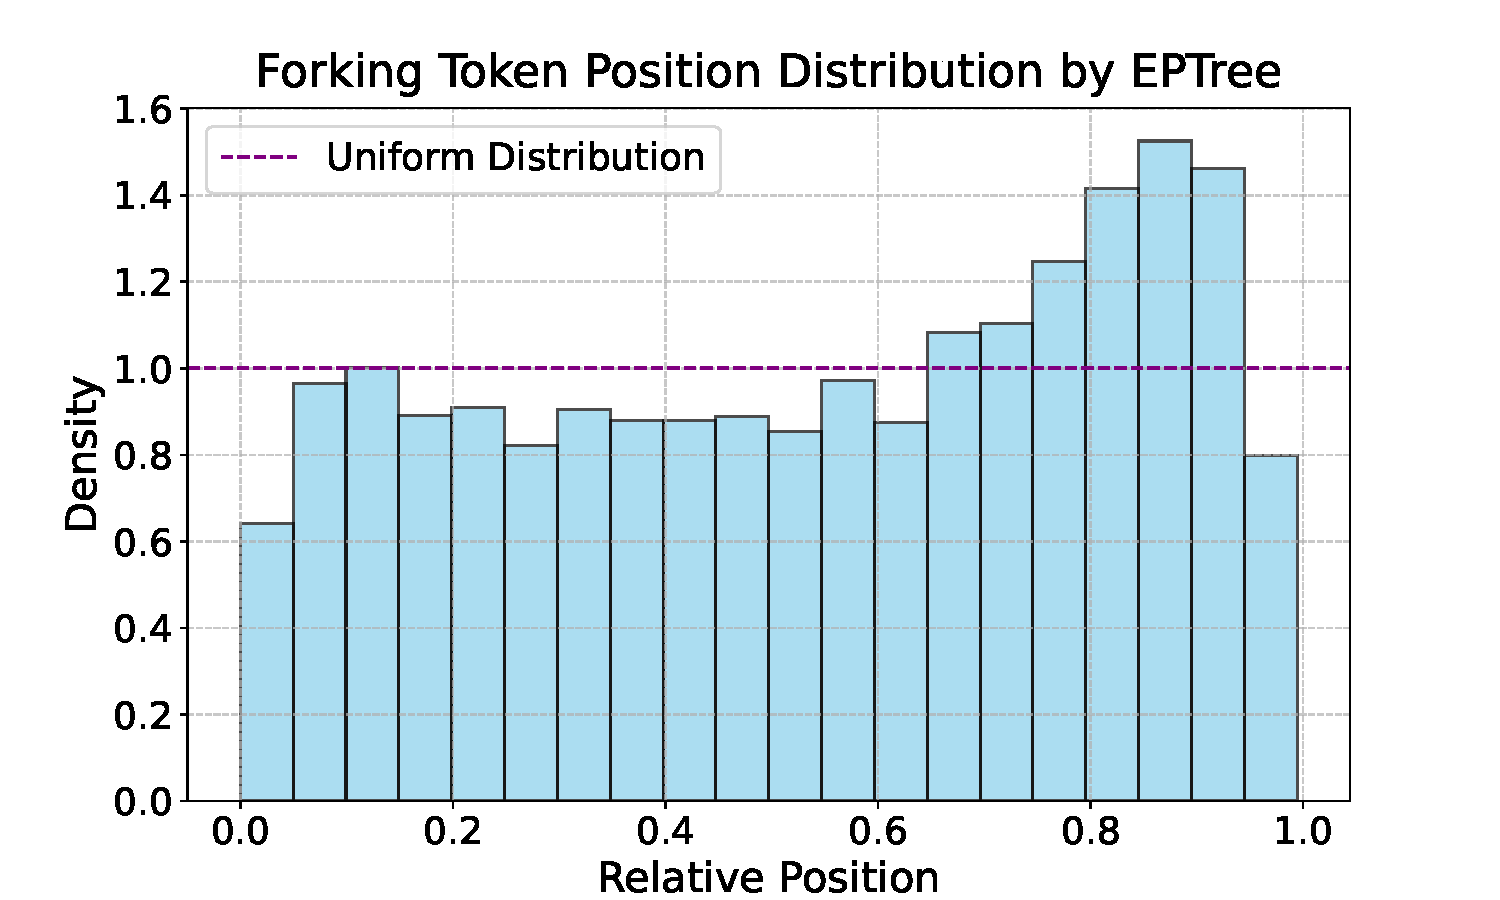
\includegraphics[width=0.9\linewidth]{figure/forked_token_position_ratio_density.pdf}
    %\caption{Position distribution of top-$20$ tokens with the highest entropy on generated responses on Omni-MATH-500.}
    \caption{Distribution of the relative positions of forking tokens selected by \treemodel on Omni-MATH-500, based on the ratio of forking position to branch length.}
    \label{fig:forked_token_position_ratio_histogram}
\end{figure}

\section{Theoritical Analysis of \treemodel}
\label{sec:appendix:proof}

\begin{theorem}
\label{thm:leaf_num_bound}
Consider a setting where forking tokens follow a uniform distribution $\mathcal{U}(0,1)$ within each branch, and generation lengths remain fixed without repetition, subject to the constraint that parameter $l \leq 2$. Under these conditions, the entropy-guided tree search algorithm presented in \Cref{sec:entropy-tree} yields a leaf count that is bounded between $\dfrac{4}{3}$ and $\dfrac{12}{5}$ times that of a multi-sampling approach, while maintaining identical computational complexity in terms of total token evaluations.
\end{theorem}


\begin{proof}
We present the proof of \Cref{thm:leaf_num_bound} by analyzing two cases based on the branching process illustrated in \Cref{fig:branching}. Let $x_1, x_2, \dots, x_n$ be i.i.d. random variables uniformly distributed on $[0,1]$.

\begin{figure}[htbp]
    \centering
    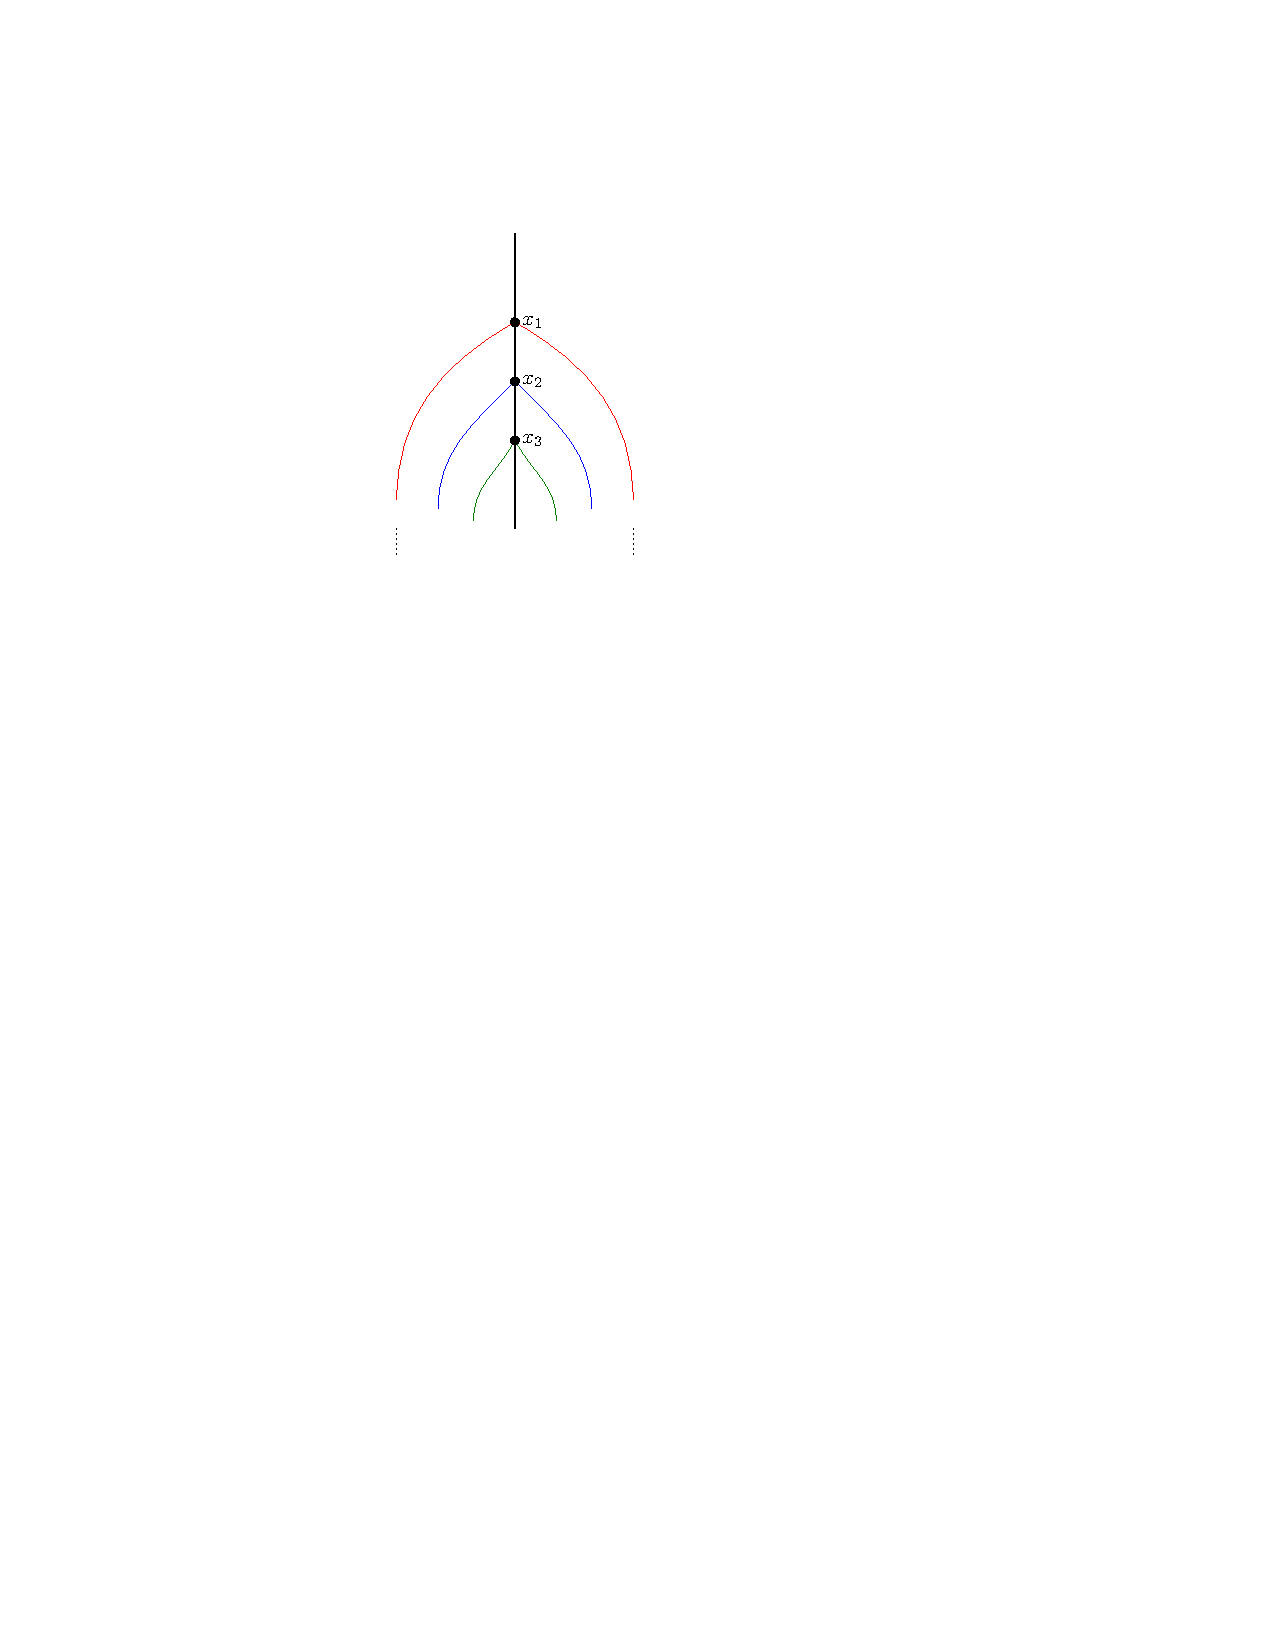
\includegraphics[width=0.95\linewidth]{figure/proof-view.pdf}
    \caption{Forking token illustration when $n=3, t=2$, where $x_1, x_2, x_3 \stackrel{\text{i.i.d}}{\sim} \mathcal{U}(0,1)$.}
    \label{fig:branching}
\end{figure}

\textbf{Case $l=1$}: Assume all completion lengths are unit $1$. The total completion length of the entropy-tree is:
\[
L = 1 + t \cdot \sum_{i=1}^n (1 - x_i).
\]
The expected total length is:
\[
\mathbb{E}[L] = 1 + t \cdot \sum_{i=1}^n \mathbb{E}[1 - x_i] = 1 + \frac{nt}{2}.
\]
The number of leaves in the tree is:
\[
N_{\text{tree}} = 1 + nt.
\]
For the multi-sample approach with the same completion tokens, the number of leaves is:
\[
N_{\text{multi}} = 1 + \frac{nt}{2}.
\]
The ratio of the number of leaves in the tree to the multi-sample approach is:
\[
R(n, t) = \frac{1 + nt}{1 + \frac{nt}{2}}.
\]
Let $x = nt \geq 1$. Then:
\[
R(x) = \frac{1 + x}{1 + \frac{x}{2}}.
\]
The derivative of $R(x)$ with respect to $x$ is:
\[
R'(x) = \frac{1}{\left(1 + \dfrac{x}{2}\right)^2} > 0,
\]
indicating that $R(x)$ is monotonically increasing. Evaluating at the endpoints:
\[
R(1) = \frac{4}{3}, \quad \lim_{x \to \infty} R(x) = 2.
\]
Thus, $R(n, t) \in \left[\dfrac{4}{3}, 2\right)$ when $l=1$.

\textbf{Case $l=2$}: In this scenario, the next top-$n$ entropy token appears either on the main chain or on one of the branches. The probabilities of these events are:
\[
\frac{1}{1+t \sum_i\left(1-x_i\right)} \quad \text{and} \quad \frac{1-x_i}{1+t \sum_i\left(1-x_i\right)},
\]
Respectively. The expected new completion length is:
\[
\mathbb{E}\left[l_i\right] = \mathbb{E}\left[\frac{\dfrac{1}{2}+\dfrac{t}{2} \sum_i\left(1-x_i\right)^2}{1+t \sum_i\left(1-x_i\right)}\right] := \varphi.
\]
Through Monte Carlo simulation, it is observed that $\varphi$ monotonically decreases with $n$. As $n \rightarrow \infty$, the ratio tends to $\dfrac{1}{3}$. For $n=1$, the integral value is $\ln 2 - \dfrac{1}{4}$. Thus, $\varphi \in \left(\dfrac{1}{3}, \ln 2 - \dfrac{1}{4}\right]$.

The total generation length is:
\[
1 + \frac{1}{2} n t + n t \cdot \varphi,
\]
And the number of leaves is:
\[
1 + 2 n t.
\]
For the same completion length, the number of leaves in the multi-sample approach is:
\[
1 + \left(\frac{1}{2} + \varphi\right) n t.
\]
The ratio of the number of leaves in the tree to the multi-sample approach is:
\[
R(nt) = \frac{1 + 2 n t}{1 + \left(\dfrac{1}{2} + \varphi\right) n t},
\]
Which is also monotonically increasing in $nt$. Therefore:
\[
R(nt) \in \left[\dfrac{6}{3 + 2\varphi}, \dfrac{4}{1 + 2\varphi}\right).
\]
Specifically:
\[
\begin{cases}
    R(nt)\geq \dfrac{6}{3+2\cdot \left(\ln 2-\dfrac{1}{4}\right)}\approx 1.544 
    \\ R(nt)<\dfrac{4}{1+2\cdot \dfrac{1}{3}}=2.4
\end{cases}
\]
Combining both cases, the ratio $R(n, t)$ lies in the interval $\left[\dfrac{4}{3}, \dfrac{12}{5}\right)$.

\end{proof}

\section{Detailed Evaluation of \treemodel}
\Cref{tab:tree-parameter-evaluation} presents a comprehensive evaluation of \treemodel in comparison to the multi-chain baseline for $k=16$. We select the RL training configuration $(6,2,1,2)$, as it offers a similar inference cost to the chain-16 setting while demonstrating improved efficiency (requiring only one interaction) and effectiveness (achieving 56.9 compared to 52.4).
\label{sec:appendix:eptree_table}
\begin{table}[!t]
    \centering
    \caption{$(M,N,L,T)$ Parameter Evaluation of \treemodel on Omni-MATH-500. The table reports the leaf number, PassRate, and total generation tokens under different parameter combinations for $k=16$ and $k=64$.}
    \label{tab:tree-parameter-evaluation}
    \resizebox{0.45\textwidth}{!}{%
        \begin{tabular}{@{}cccccc@{}}
            \toprule[1.2pt]
            \multicolumn{1}{c}{$\textbf{(M, N, L, T)}$} & \textbf{\#Leaf} $\uparrow$ & \textbf{PassRate} $\uparrow$ & \textbf{\#Token} $\downarrow$ \\
            \midrule
            \multicolumn{4}{c}{\textit{$k=16$}} \\
            \midrule
            multi-16      & 16 & 52.4 & 19858 \\
            (8, 3, 1, 1)  & 32 & 58.4 & 25223 \\
            (7, 2, 1, 2)  & 35 & 59.2 & 26200 \\
            (6, 2, 2, 1)  & 30 & 54.4 & 20537 \\
            (6, 2, 1, 2)  & 30 & 56.9 & 22268 \\
            (5, 3, 1, 2)  & 35 & 58.6 & 25269 \\
            (5, 2, 1, 3)  & 35 & 56.0 & 25210 \\
            (5, 3, 2, 1)  & 35 & 58.0 & 22668 \\
            (5, 1, 2, 3)  & 35 & 58.6 & 21895 \\
            \midrule
            \multicolumn{4}{c}{\textit{$k=64$}} \\
            \midrule
            multi-64      & 64 & 67.4 & 79367 \\
            (16, 2, 2, 2) & 144 & 70.0 & 88257 \\
            (16, 4, 1, 2) & 144 & 71.4 & 101744 \\\
            (16, 2, 1, 4) & 144 & 72.6 & 100468 \\
            (9, 5, 1, 3)  & 144 & 71.9 & 98193 \\
            (9, 3, 1, 5)  & 144 & 71.6 & 97193 \\
            (8, 8, 1, 2)  & 136 & 70.7 & 92946 \\
            (8, 4, 1, 4)  & 136 & 69.7 & 90015 \\
            (8, 8, 2, 1)  & 136 & 68.6 & 79582 \\
            (8, 4, 2, 2)  & 136 & 71.0 & 77768 \\
            (8, 2, 2, 4)  & 136 & 69.4 & 76750 \\
            \bottomrule[1.2pt]
        \end{tabular}
    }
\end{table}

\section{Results on Other Reasoning Benchmarks}
Figure \ref{fig:qwen_results_appendix} and  \ref{fig:glm_results_appendix} provide additional RL training results on MATH500, AMC, LiveCodeBench, and AIME2024, demonstrating that \model with \treemodel sampling outperforms RL with traditional multi-chain sampling across various benchmarks. 
\label{sec:appendix:other_benchmark}
\begin{figure*}[htbp]
    \centering
        \begin{minipage}{\textwidth}
            \centering
            \begin{minipage}{0.4\textwidth}
                \centering
                
\includegraphics[width=\textwidth]{figure/qwen-rlresult/math.pdf}
                \vspace{-5mm}
                \label{fig:first_image_app}
            \end{minipage}
            \hfill
            \begin{minipage}{0.4\textwidth}
                \centering
                
\includegraphics[width=\textwidth]{figure/qwen-rlresult/amc.pdf}
                \vspace{-5mm}
                \label{fig:second_image_app}
            \end{minipage}
            \vspace{1mm}
            \\
            \begin{minipage}{0.4\textwidth}
                \centering
                
\includegraphics[width=\textwidth]{figure/qwen-rlresult/lcb.pdf}
                \vspace{-5mm}
                \label{fig:third_image_app}
            \end{minipage}
            \hfill
            \begin{minipage}{0.4\textwidth}
                \centering
                
\includegraphics[width=\textwidth]{figure/qwen-rlresult/aime2024.pdf}
                \vspace{-5mm}
                \label{fig:fourth_image_app}
            \end{minipage}
        \end{minipage}
    \caption{Performance comparison between \model and ChainRL on MATH500 (Upper Left), AMC (Upper Right), LiveCodeBench (Lower Left), and AIME2024 (Lower Right); experiments are based on Qwen-2.5-14B.}
    \label{fig:qwen_results_appendix}
\end{figure*}

\vspace{1mm}

\begin{figure*}[htbp]
    \centering
        \begin{minipage}{\textwidth}
            \centering
            \begin{minipage}{0.4\textwidth}
                \centering
                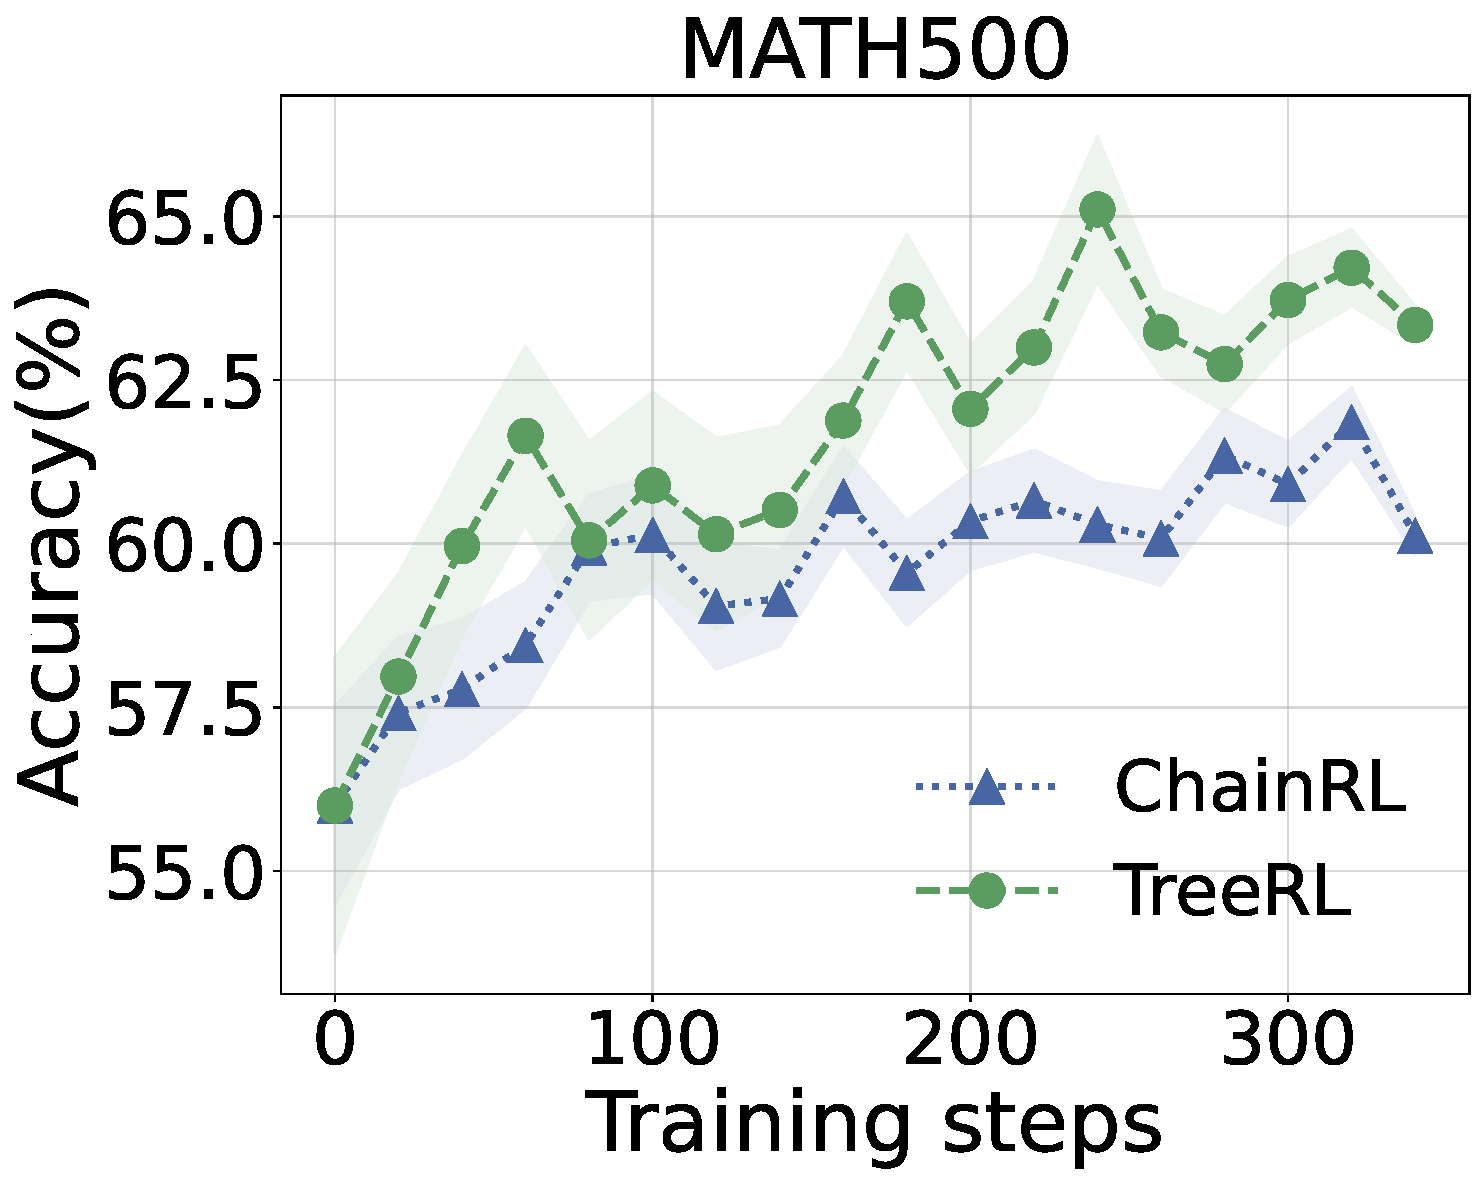
\includegraphics[width=\textwidth]{figure/glm-rlresult/math.pdf}
                \vspace{-5mm}
                \label{fig:fifth_image}
            \end{minipage}
            \hfill
            \begin{minipage}{0.4\textwidth}
                \centering
                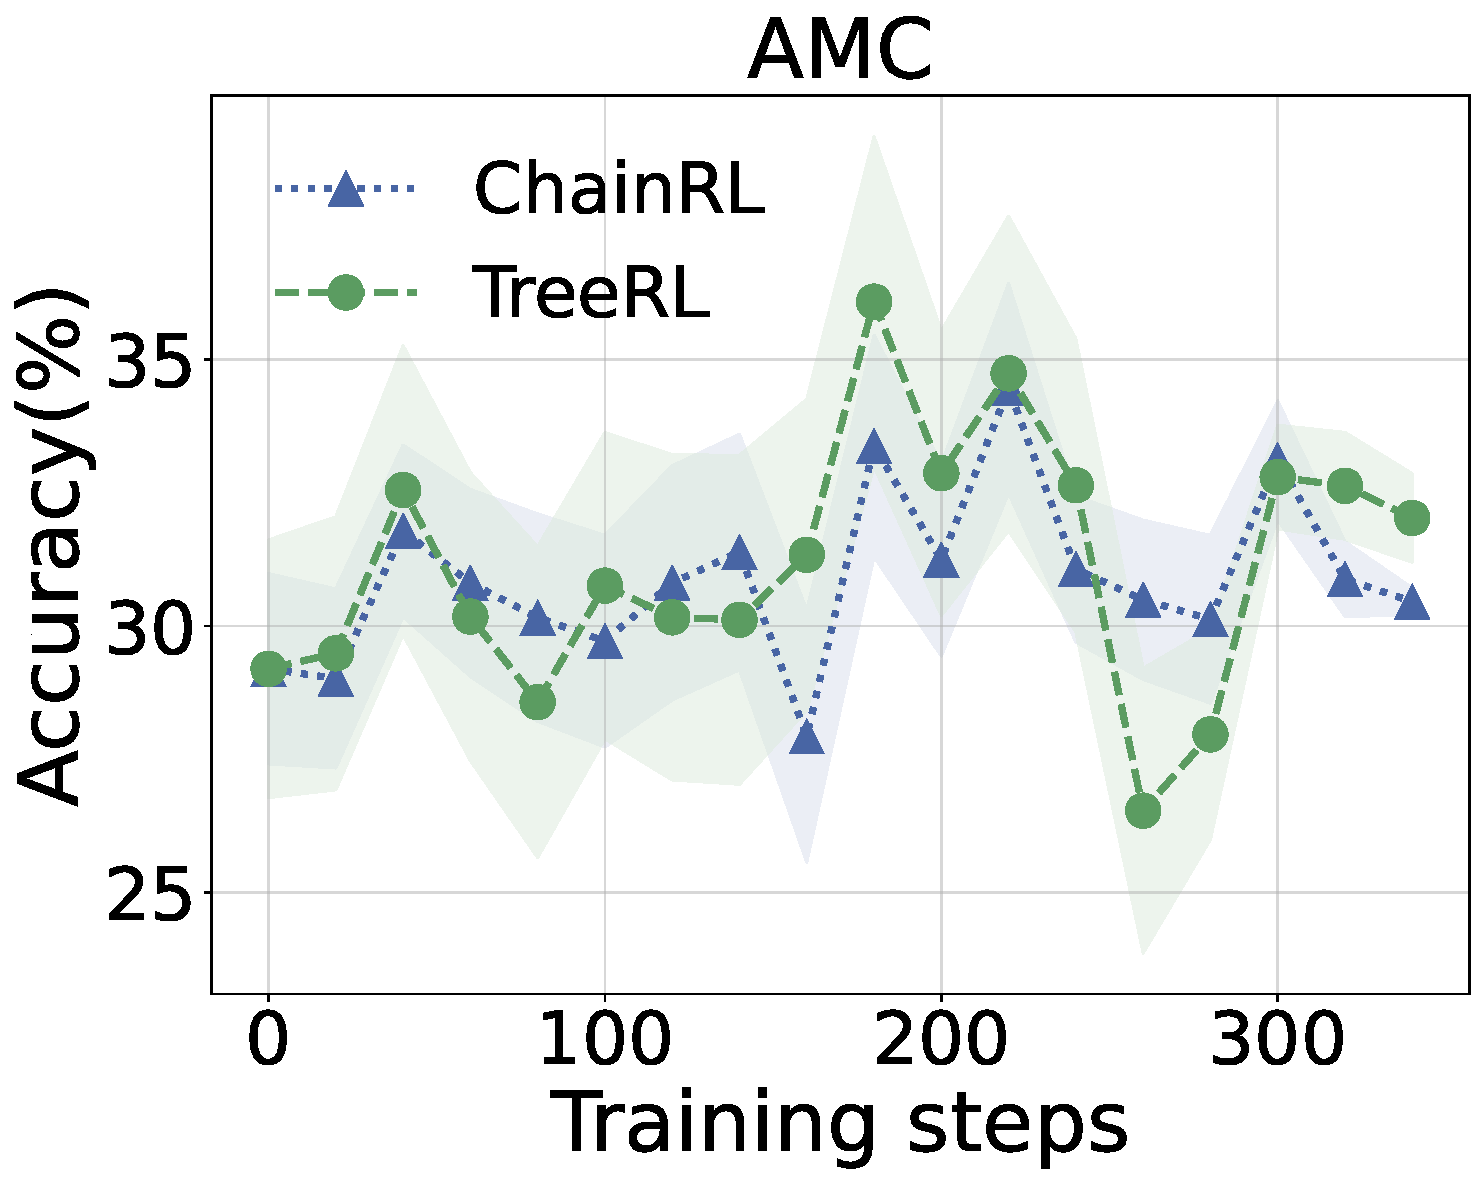
\includegraphics[width=\textwidth]{figure/glm-rlresult/amc.pdf}
                \vspace{-5mm}
                \label{fig:sixth_image_app}
            \end{minipage}
            \vspace{1mm}
            \\
            \begin{minipage}{0.4\textwidth}
                \centering
                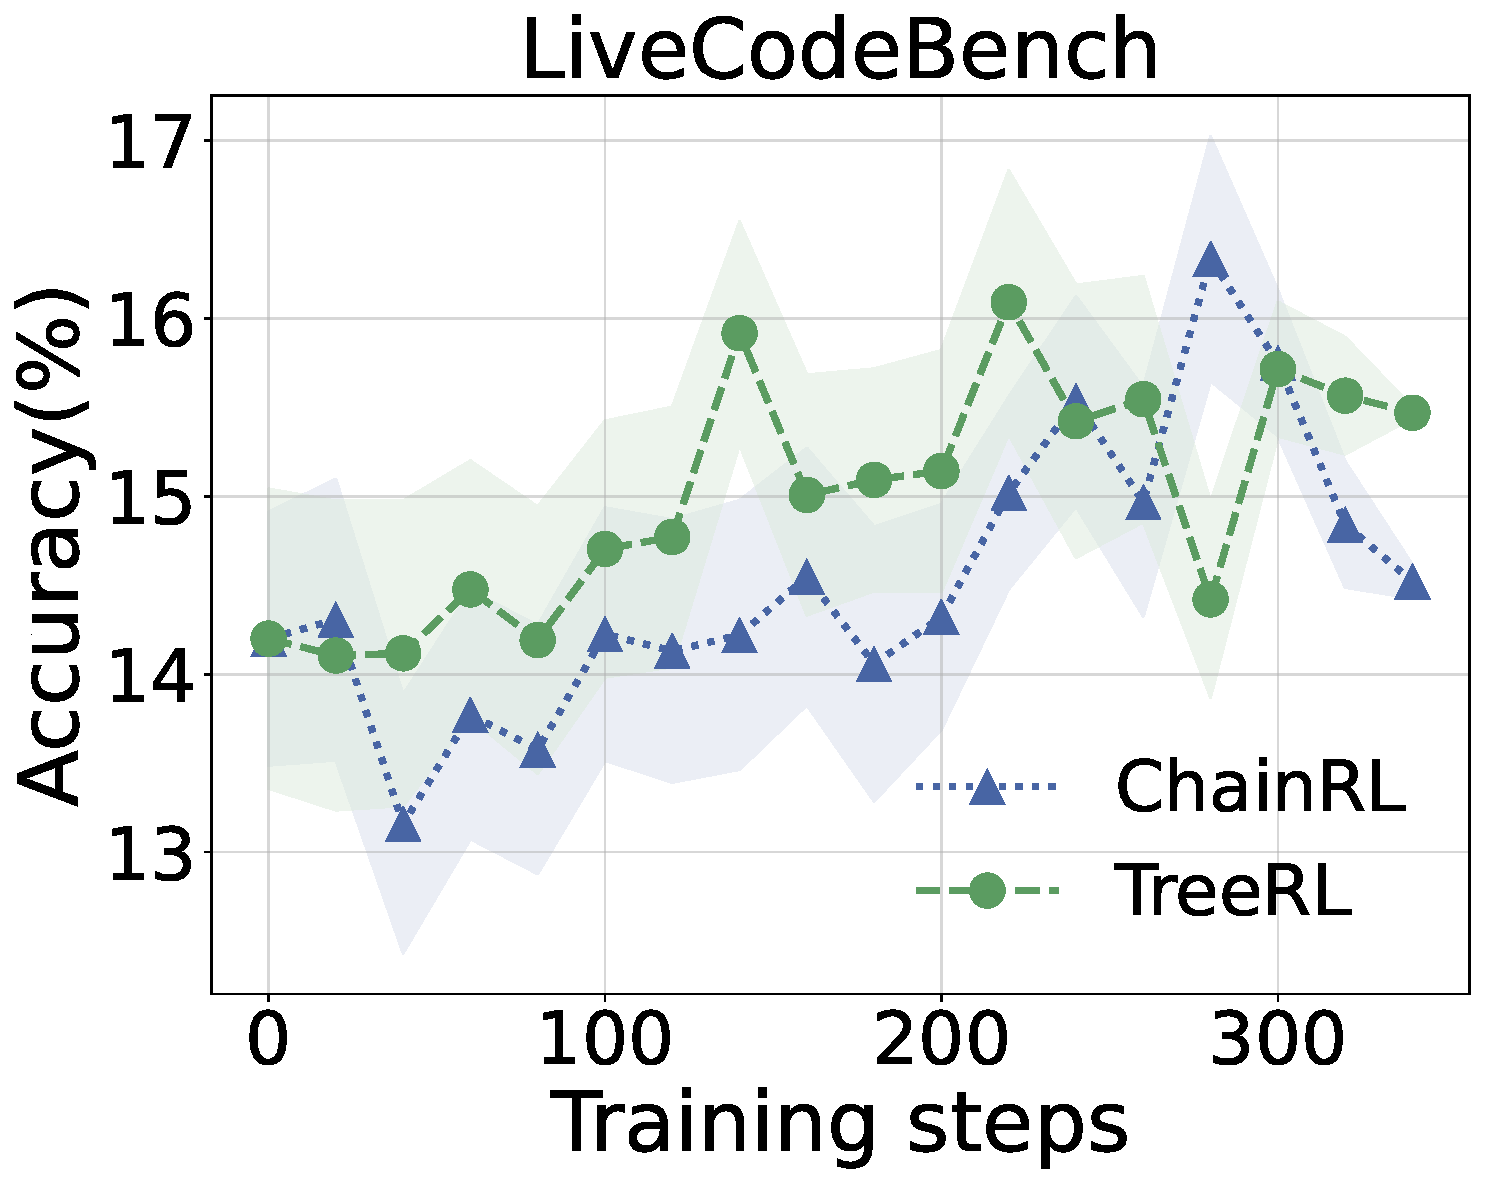
\includegraphics[width=\textwidth]{figure/glm-rlresult/lcb.pdf}
                \vspace{-5mm}
                \label{fig:seventh_image}
            \end{minipage}
            \hfill
            \begin{minipage}{0.4\textwidth}
                \centering
                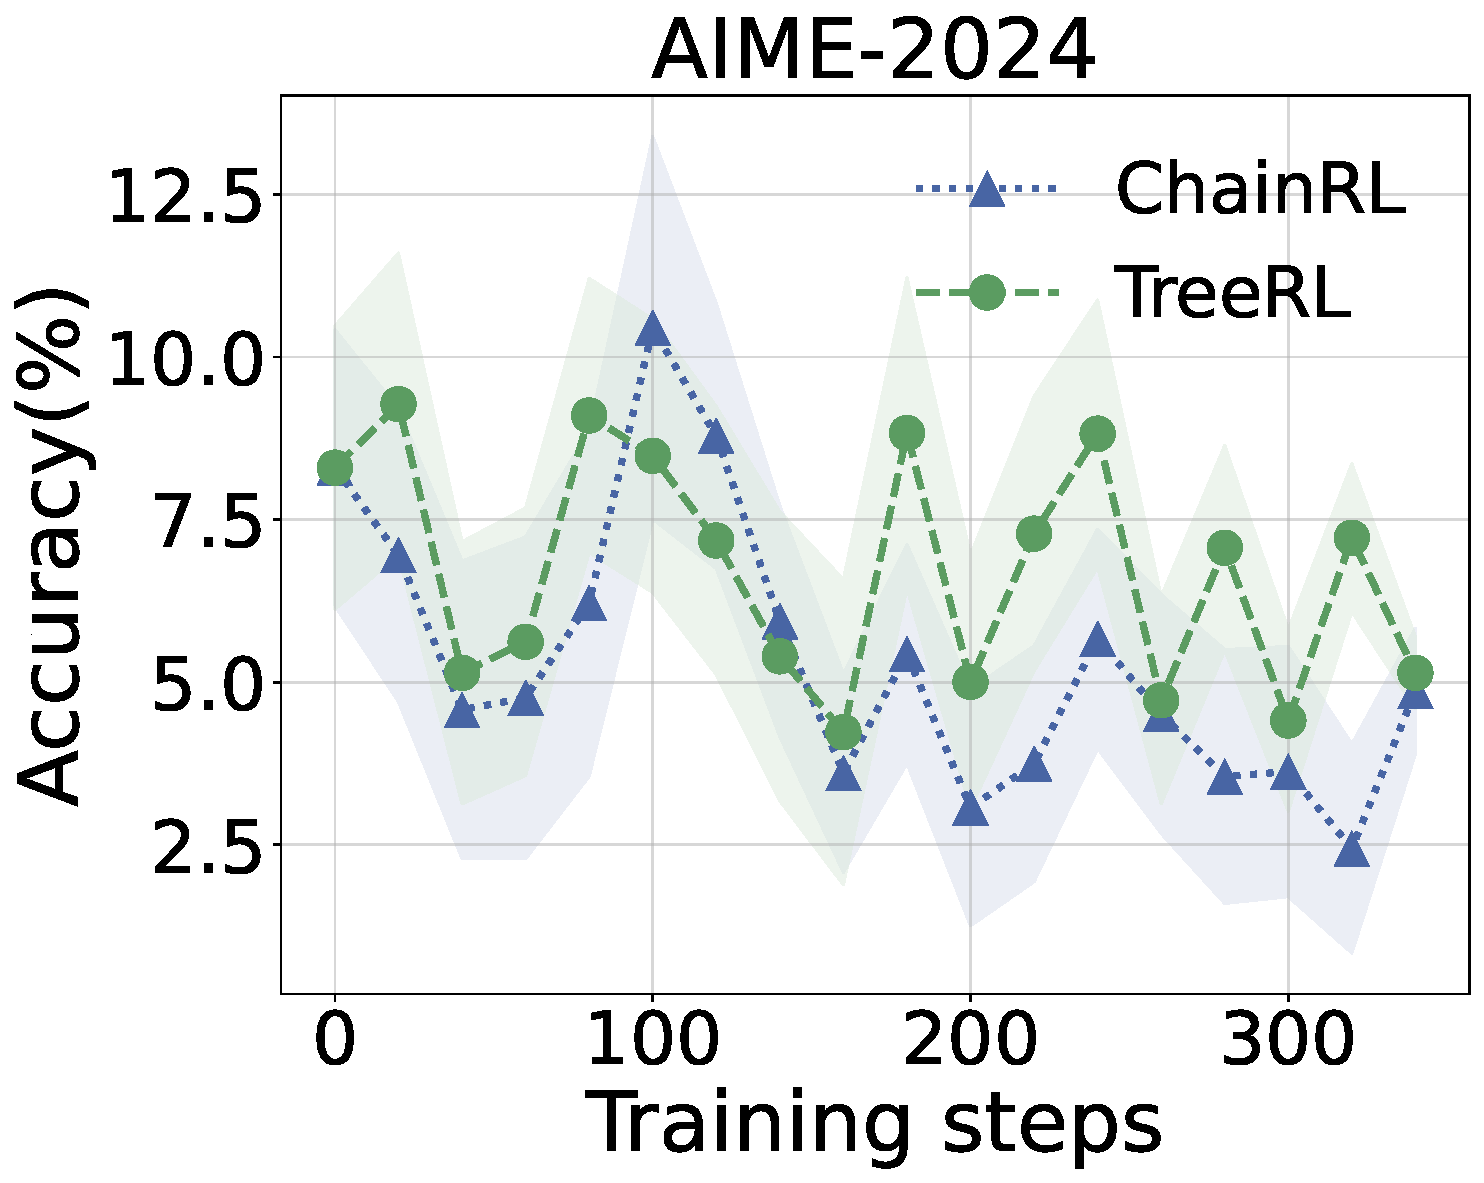
\includegraphics[width=\textwidth]{figure/glm-rlresult/aime2024.pdf}
                \vspace{-5mm}
                \label{fig:eighth_image}
            \end{minipage}
        \end{minipage}
    \caption{Performance comparison between \model and ChainRL on MATH500 (Upper Left), AMC (Upper Right), LiveCodeBench (Lower Left), and AIME2024 (Lower Right); experiments are based on GLM4-9B.}
    \label{fig:glm_results_appendix}
\end{figure*}

\section{\model on General tasks}

% We also evaluate our algorithm on general tasks. First, we fine-tune the Qwen-2.5-14B model using a dataset mixed with reasoning and general tasks. Then, we run both \model and ChainRL. For this experiment, we use the hyperparameter setting of $(6,2,1,2)$ for \model and set $k=16$ for ChainRL. General instruction data is employed for RL training, with ORM serving as the signal, as designing a rule-based reward for general responses is challenging. All other settings are consistent with those described in \Cref{sec:exp_setup}. We evaluate the \model on $3$ general tasks: MMLU-Pro~\citep{wang2024mmlu}, Arena-Hard~\citep{li2024crowdsourced}, and IFEval~\citep{zhou2023instruction}.
To further evaluate \model's generalizability, we further conducted experiments on general tasks.
We evaluate \model and ChainRL on $3$ general tasks: MMLU-Pro~\citep{wang2024mmlu}, Arena-Hard~\citep{li2024crowdsourced}, and IFEval~\citep{zhou2023instruction}.

\begin{itemize}
    \item MMLU-Pro extends MMLU~\citep{hendrycks2020measuring} with more challenging reasoning tasks, fewer noisy questions, and a larger answer set (4-10 options). We use the chain-of-thought prompt and measure the pass rate.
    \item Arena-Hard consists of 500 difficult prompts from Chatbot Arena, focusing on human-like preferences. We evaluate using the win rate score, comparing against the GPT-4-0314 baseline.
    \item IFEval tests the model's ability to follow prompt instructions. We use the strict prompt metric for evaluation.
\end{itemize}

\begin{table}[ht]
    \centering
    \resizebox{\linewidth}{!}{
        \begin{tabular}{lcccc}
        \toprule[1.2pt]
             &  MMLU-Pro & Arena-hard & IFEval & Avg\\
        \midrule
            SFT     & 57.6 & 57.5 & 49.9 & 55.0 \\
            ChainRL & 64.5 & 72.2 & 56.0 & 64.2 \\
            \model  & 64.5 & 71.8 & 58.2 & 64.9 \\
        \bottomrule[1.2pt]
        \end{tabular}
    }
    \caption{Performance on general benchmarks.}
    \label{tab:general-task-performance}
\end{table}

% As shown in \Cref{tab:general-task-performance}, \model does not outperform ChainRL on the general tasks.

As is shown in \Cref{tab:general-task-performance}, we observe a comparable performance between \model and ChainRL. This indicates that while \model exhibits a particular advantage in reasoning tasks, it maintains its performance in general tasks, achieving robust performance in diverse task types.

